\documentclass[10pt,twocolumn,letterpaper]{article}

\usepackage{cvpr}
\usepackage{times}
\usepackage{epsfig}
\usepackage{graphicx}
\usepackage{amsmath}
\usepackage{amssymb}

% Include other packages here, before hyperref.

% If you comment hyperref and then uncomment it, you should delete
% egpaper.aux before re-running latex.  (Or just hit 'q' on the first latex
% run, let it finish, and you should be clear).
\usepackage[pagebackref=true,breaklinks=true,letterpaper=true,colorlinks,bookmarks=false]{hyperref}

% \cvprfinalcopy % *** Uncomment this line for the final submission

\def\cvprPaperID{2254} % *** Enter the CVPR Paper ID here
\def\httilde{\mbox{\tt\raisebox{-.5ex}{\symbol{126}}}}

% Pages are numbered in submission mode, and unnumbered in camera-ready
\ifcvprfinal\pagestyle{empty}\fi
\begin{document}

%%%%%%%%% TITLE
\title{Coupling Uncertain Active Constellation Models with \\
Cascaded Forest Predictors for Sematic Segmentation \\ -- Supplement --}

\author{First Author\\
Institution1\\
Institution1 address\\
{\tt\small firstauthor@i1.org}
% For a paper whose authors are all at the same institution,
% omit the following lines up until the closing ``}''.
% Additional authors and addresses can be added with ``\and'',
% just like the second author.
% To save space, use either the email address or home page, not both
\and
Second Author\\
Institution2\\
First line of institution2 address\\
{\tt\small secondauthor@i2.org}
}

\maketitle
%\thispagestyle{empty}

%%%%%%%%% ABSTRACT
%\begin{abstract}
The following supplemental results provide additional insights that support the results given and discussed in the paper. 
%
We will include Figures~\ref{fig:var-importance}~and~\ref{fig:output-over-levels} of this supplement into the paper. 

%\end{abstract}
\section{Variable Importance}
We evaluated \emph{variable importance}~\cite{BreimanRF} for our approach (Figure~\ref{fig:var-importance}, left) as well as the MAP approach (Figure~\ref{fig:var-importance}, right). 
%%
Variable importance measures how much worse a forest would perform (as a fraction of 1) with a random feature instead of the feature corresponding to the respective variable -- in other words, variable importance captures how important a feature is for the performance of a forest. 
%
Figure~\ref{fig:var-importance} lists the aggregated (i.e.\ summed) variable importance the three classes of features we employ, namely filter bank features (1st column), RF output (2nd column), and smoothed RF output (3rd column). Note that RF output and smoothed RF output are not available on the first level. 
%
Figure~\ref{fig:var-importance} reveals how important the smoothed RF output is for forest performance in our approach (Level 2: 0.55, Level 3: 0.46), as opposed to the MAP approach, where the smoothed RF output is considerably less important (Level 2: 0.24, Level 3: 0.25). 
%
%
\begin{figure*}[h!]
\begin{center}
\begin{tabular}{cc}
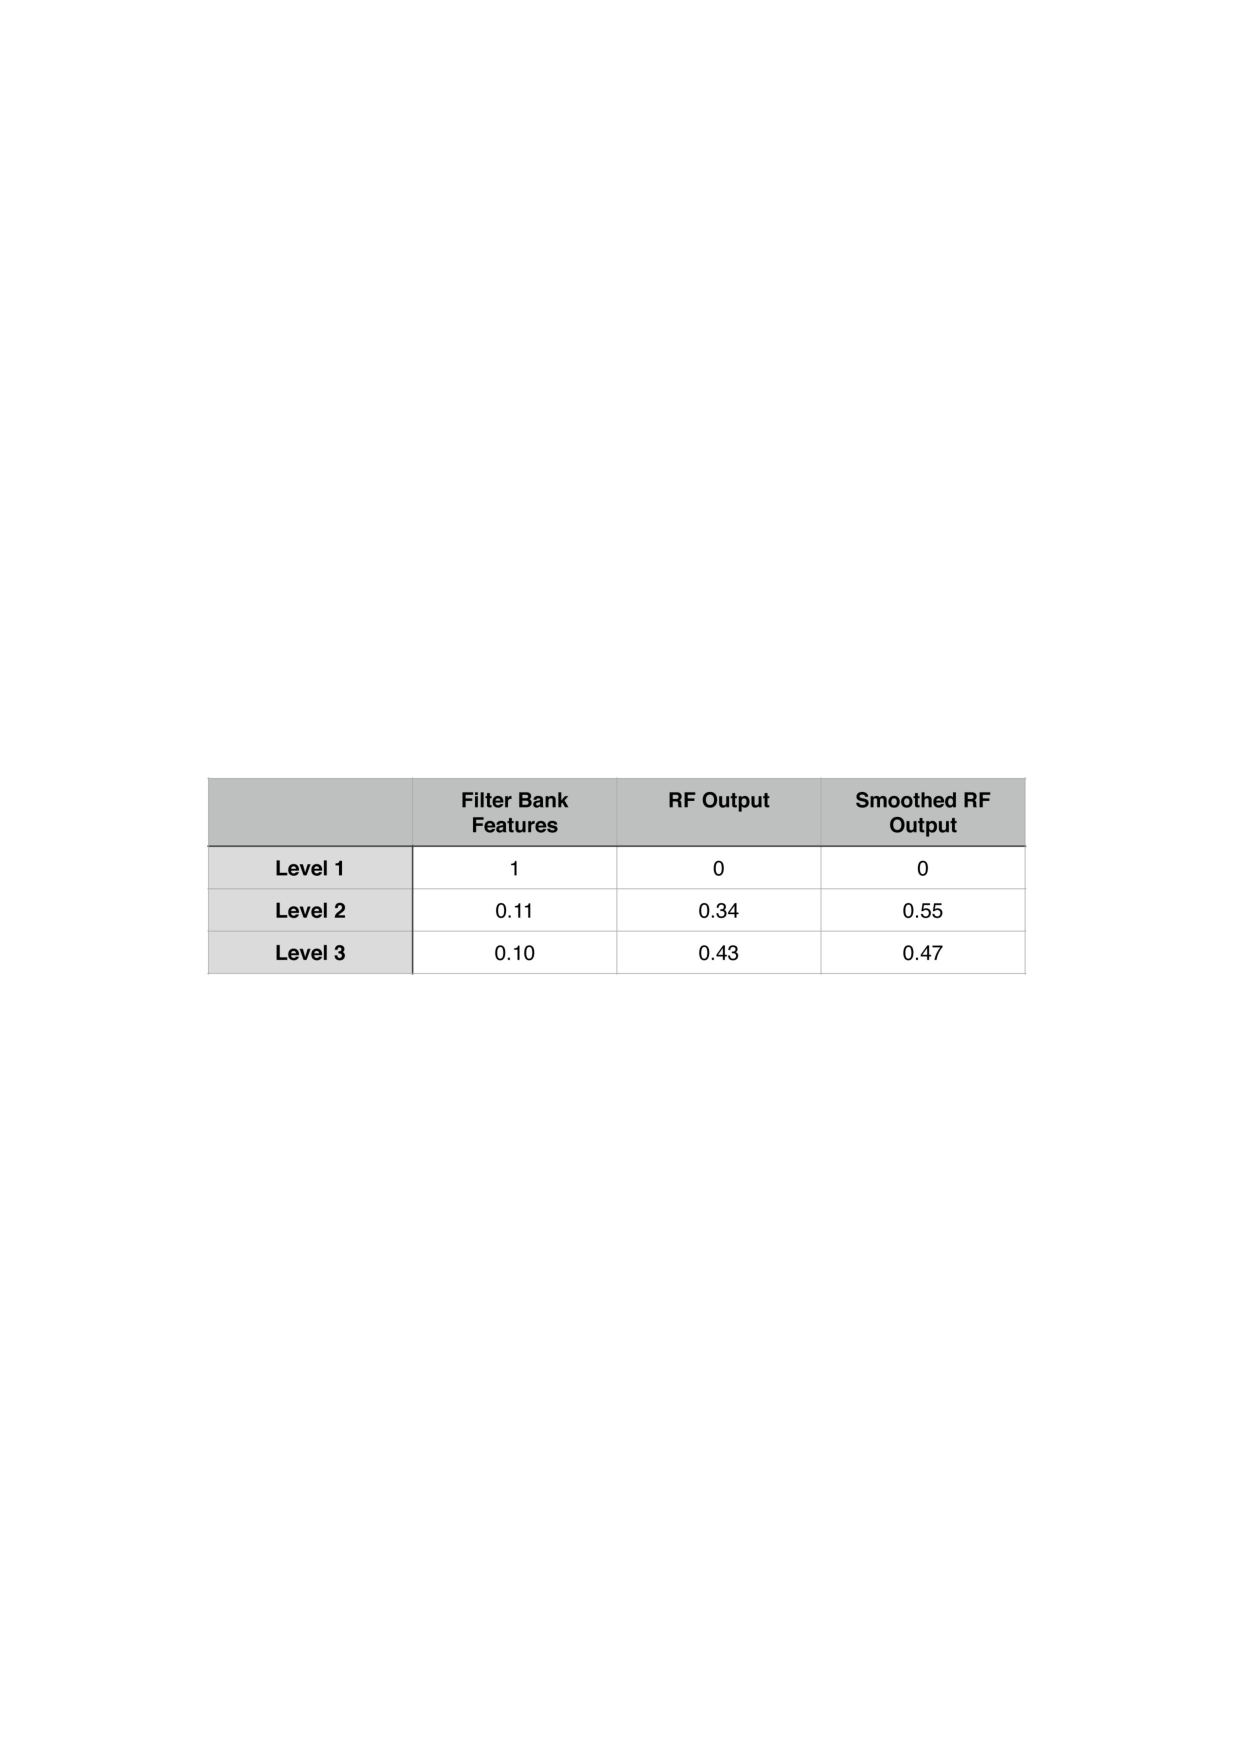
\includegraphics[width=\columnwidth]{VariableImportance_Ours.jpg} &
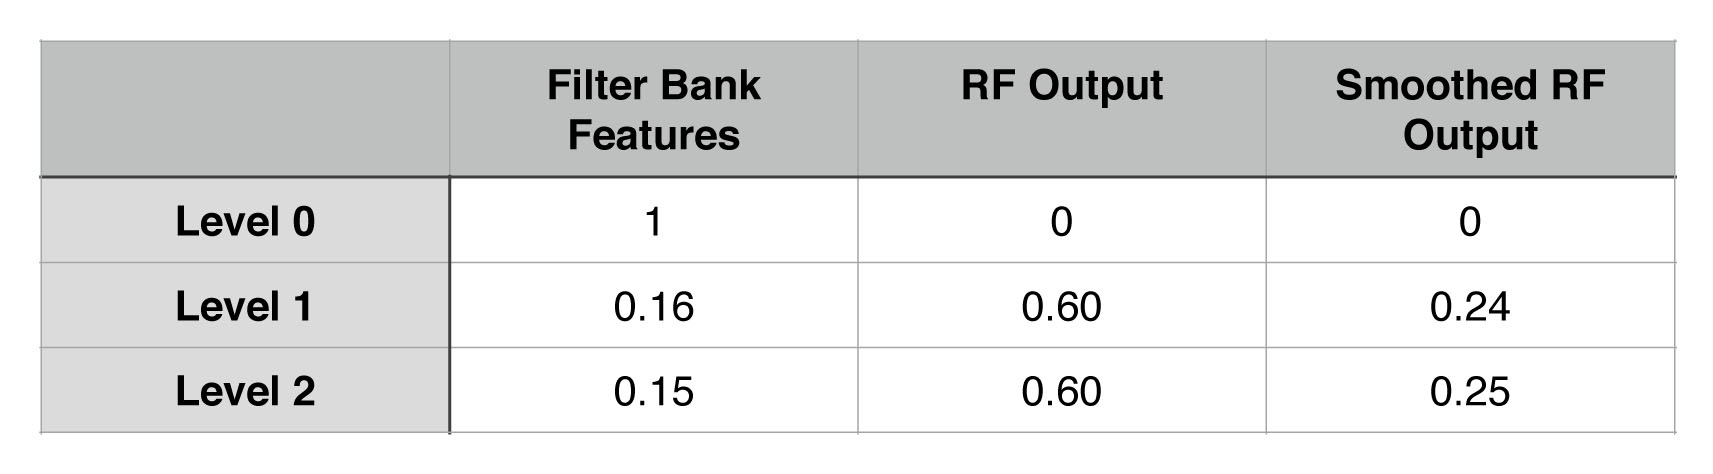
\includegraphics[width=\columnwidth]{VariableImportance_MAP.jpg} \\
Our approach: Marginals for smoothing RF output & MAP instead of marginals \\
\end{tabular}
\caption{Variable importance. Variable importance reveals that smoothed RF output in the form of marginals is much more beneficial for the performance of the forest than the alternative MAP solution. }
\label{fig:var-importance}
\end{center}
\end{figure*}

\section{Additional Exemplary Results}
%
\begin{figure*}[t]
\begin{center}
%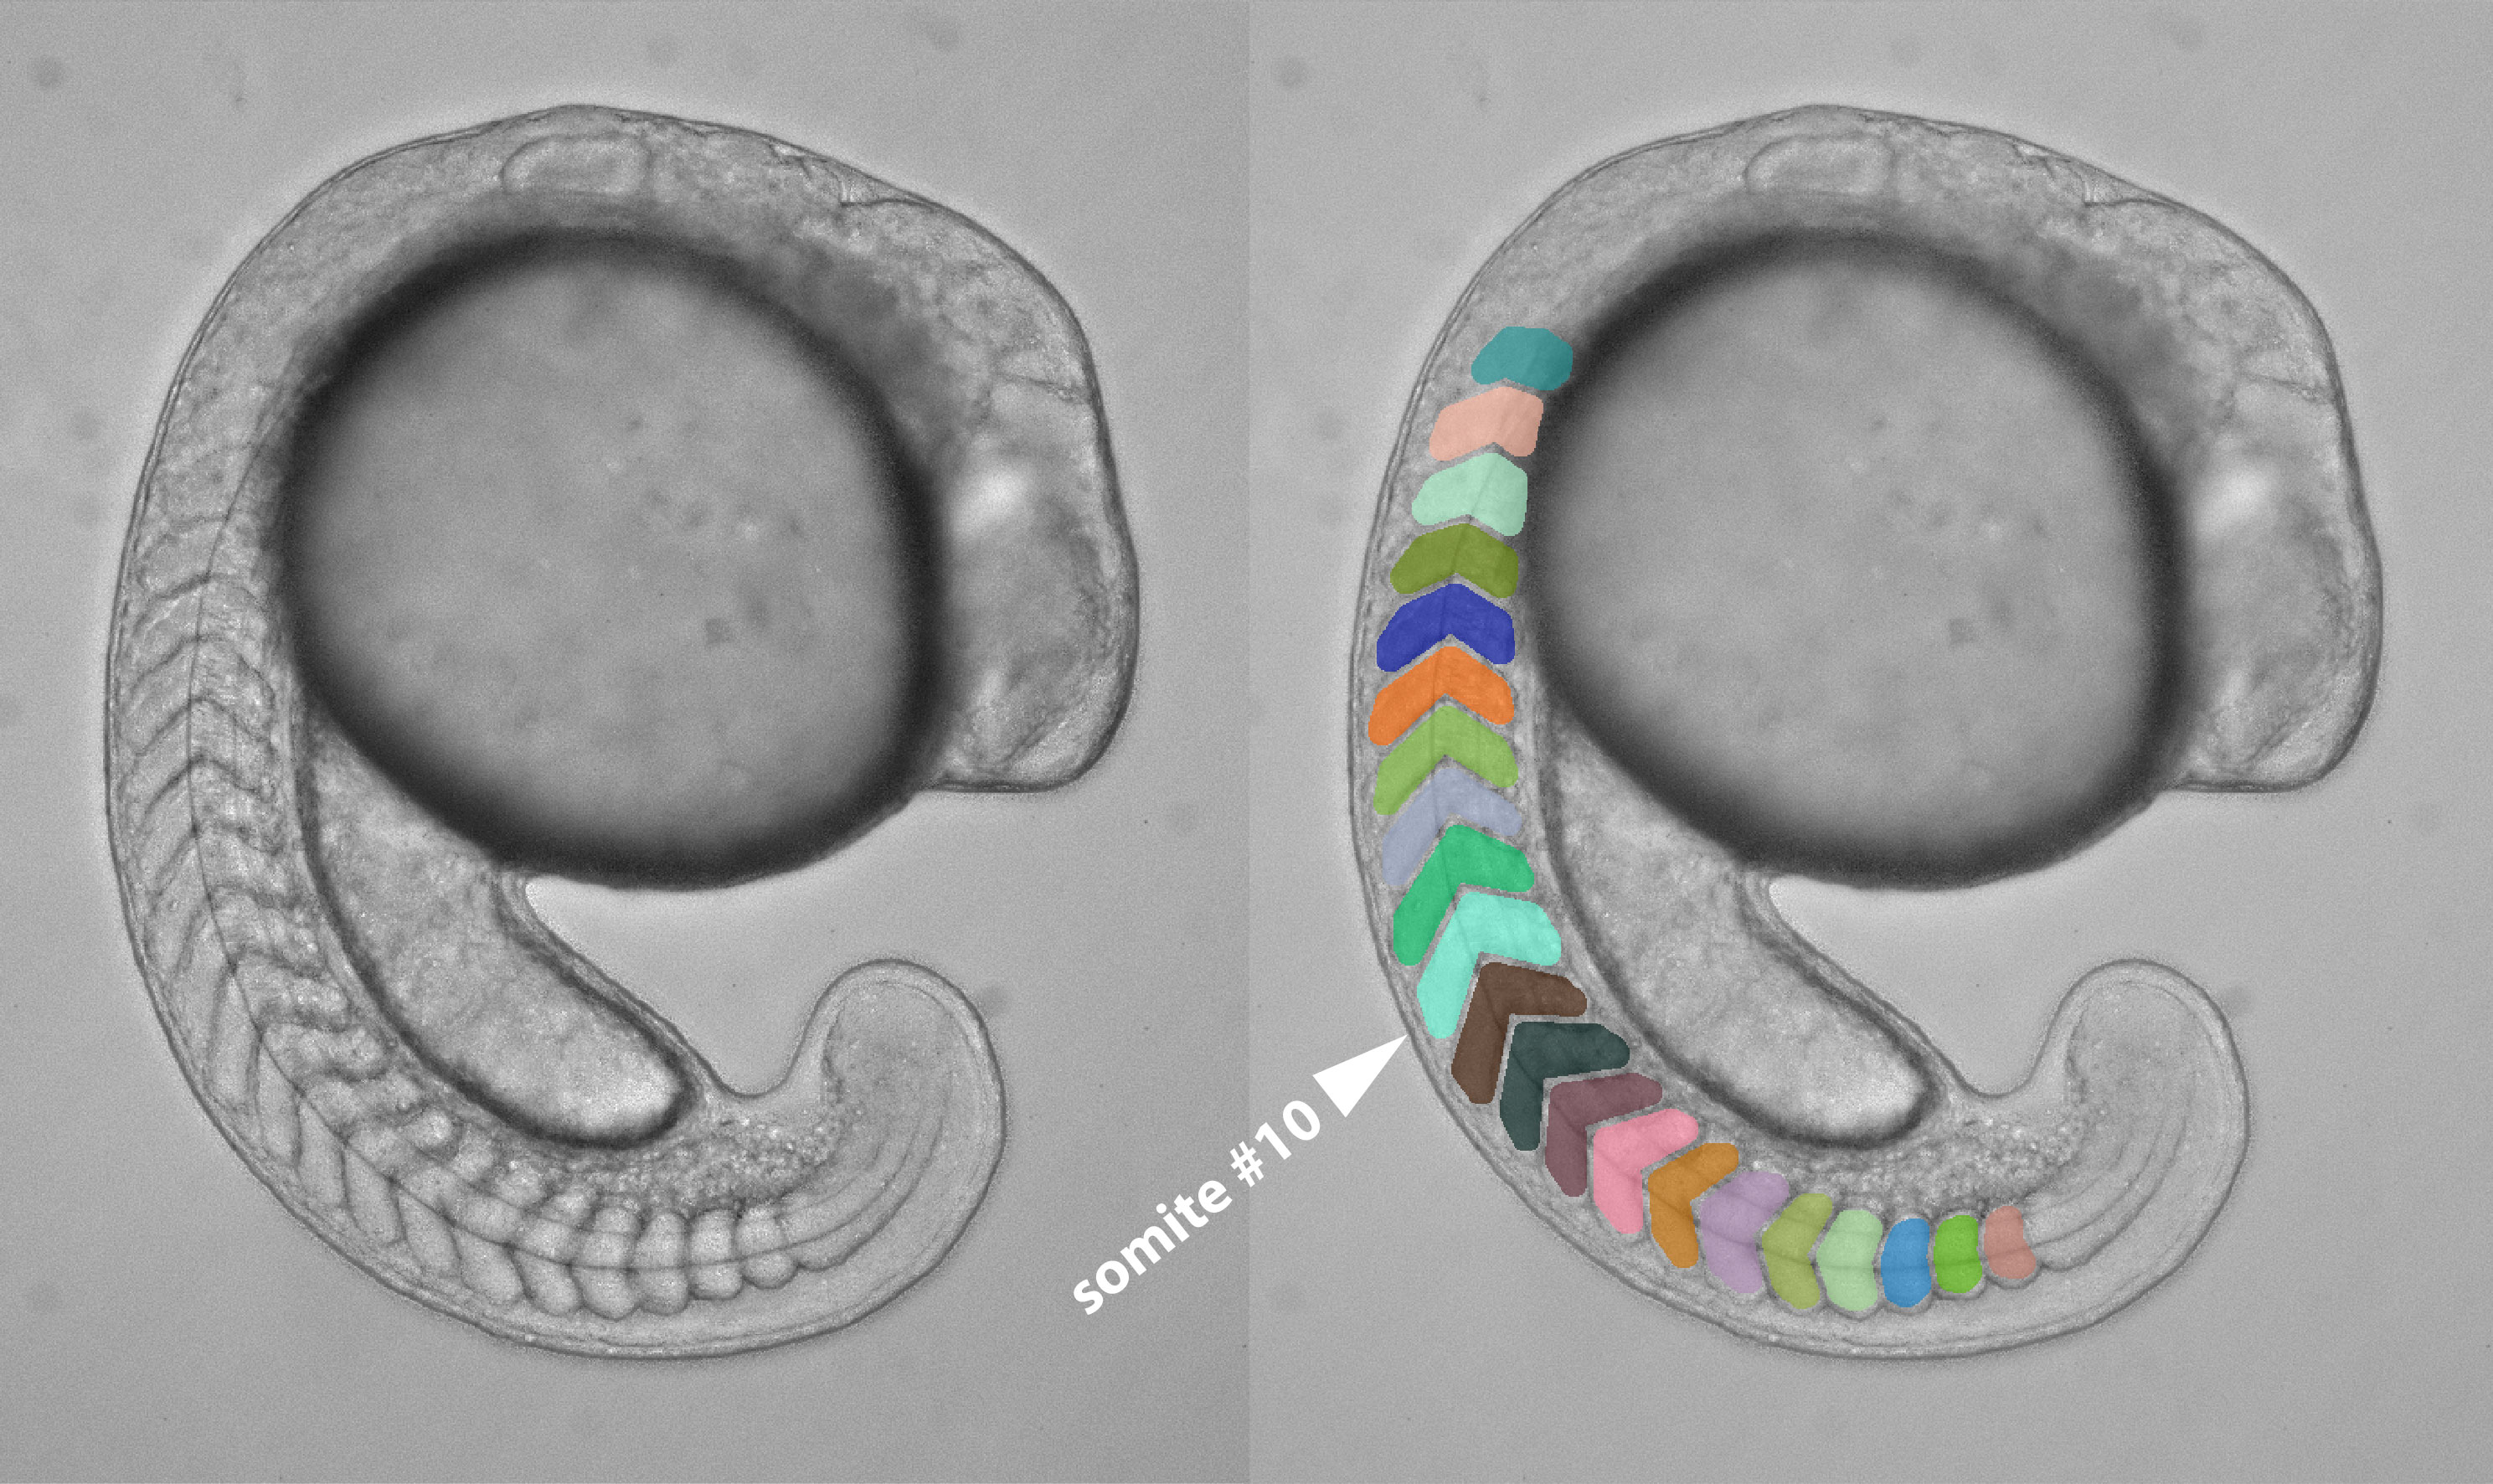
\includegraphics[width=\columnwidth]{TopRight.jpg} 
\caption{Output and smoothed output over levels }
\label{fig:output-over-levels}
\end{center}
\end{figure*}

{\small
\bibliographystyle{ieee}
\bibliography{somites2014-supplement}
}

\end{document}
